\problemname{Tycho}

\illustration{.4}{img/MarsPerseveranceRover.jpg}{}

\noindent
Planeedikulgur \emph{Tycho VIII} peab pärast mineraaliproovide kogumist tagasi kodubaasi saama.
Tycho liigub sirgjooneliselt positsioonilt~$0$ kodubaasi positsioonil~$b$.
Kulgur liigub aeglase, kuid ühtlase kiirusega: $1$~ühik sekundis.
Iga sekund saab planeedi karmi keskkonna tõttu Tycho $1$~ühikut kahju. 

Olukord on veelgi hullem lähedal asuva pulsari kiirguse tõttu, mis teeb iga $p$ sekundi tagant kulgurile
$d$ ühikut kahju.
Kiirgusest tulenevat kahju saab aga vältida, kui varjuda ühte $n$ erinevast varjupaigast ---koopad, taimkate, suured kivid, planeedi megafauna karkassid---mis tee peale jäävad.
Tycho võib mistahes punktis mistahes täisarvulise arvu sekundeid paigal püsida.

Alguspunkt~$0$ ja kodubaas~$b$ on mõlemad varjupaigad, seega Tycho seal kiirgusest kahju ei saa,

\medskip
Mis on vähim kahju, mida Tycho saab oma teekonnal kodubaasi saada?

\section*{Näide}

Vaatleme olukorda, kus kodubaas on positsioonil $18$ ja varjupaigad on positsioonidel $8$ ja $15$.

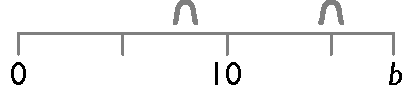
\includegraphics[width=.3\textwidth]{img/samplesetup}

Eeldame, et pulsari periood on $4$ ehk varjupaigas olemata saaks Tycho kiirgusest kahju
aegadel $4$, $8$, $12$ jne.
Kui Tycho lahkub alguspunktist (mis läheb ka varjupaigana arvesse) ajahetkel $0$, jõuab ta esimese
varjupaigani pärast $8$ sekundit ja saab seejuures ajahetkel $4$ $d$ ühikut kiirguskahju
(kuid mitte ajahetkel $8$, sest tol hetkel on ta varju all).
Peatumata jätkates jõuab ta kodubaasi ajahetkel $18$ ja saab täiendava $d+d$ kiirguskahju
(vastavalt ajahetkedel $12$ ja $18$).
Nii toimides saab kulgur $d+d+d=3d$ ühikut kiirguskahju ja $18$ ühikut kahju keskkonnalt.
Kui aga Tycho ootab $1$ sekundi teises varjupaigas (positsioonil $15$), ei saa ta kiirguskahju
ajahetkel $16$ ja jõuab kodubaasi ajahetkel $19$ võttes kokku $2d + 19$ ühikut kahju.
Enamiku $d$ väärtuste korral on see parem.
Need kaks olukorda on kujutatud alloleval joonisel.

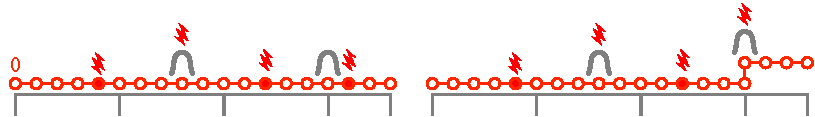
\includegraphics[width=.8\textwidth]{img/sample1_2.pdf}

Kui pulsari periood on $10$, saab Tycho alguspunktis oodata $2$~sekundit ja siis minna koju
ilma kusagil peatumata.
Niiviisi möödub ta esimesest varjupaigast (ikka positsioonil~$8$) täpselt sel hetkel, kui pulsar
kahju teeks, ja jõuab kodubaasi ajahetkel $20$. Nii saab ta kokku $20$ ühikut keskkonnalt ja mitte
ühtegi kiirguselt.

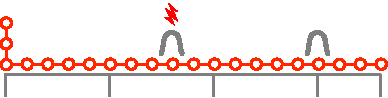
\includegraphics[width=.4\textwidth]{img/sample3.pdf}

\section*{Sisend}

Sisendi esimesel real on neli tühikutega eraldatud täisarvu $b$, $p$, $d$ ja $n$:
kodubaasi asukoht $b$,
pulsari periood~$p$,
pulsari iga sähvatuse põhjustatud kiirguskahju hulk~$d$,
varjupaikade arv~$n$.
Järgneval $n$~real on igaühel täisarv. Need kirjeldavad varjupaikade asukohti
$a_1$, $\ldots$, $a_n$, kus $0<a_1<\cdots <a_n< b$. % constraint:shelterbounds, constraint:sortedshelters

\section*{Väljund}

Trüki välja üksainus täisarv: vähim võimalik kogus kahju, millega Tycho saab jõuda positsioonini $b$.

\section*{Piirangud ja hindamine}

Võib eeldada, et
$1\leq p < b$ % constraint:pulsehappens
ja
$0 \leq n < b$. % constraint:sheltersfit
Alati kehtivad
$1\leq b\leq 10^{12}$, % constraint:b
$0\leq d \leq 10^6$, %constraint:d
ja
$0\leq n \leq 10^5$. % constraint:n

Selles ülesandes on testid jagatud gruppidesse, iga grupp on väärt mingi arvu punkte.
Iga grupi eest saavad punkte vaid need lahendused, mis läbivad kõik sellesse gruppi kuuluvad testid.
Sinu lõplik skoor on esituste maksimum.

\medskip
\begin{tabular}{lll}
Grupp & Punktid & Lisapiirangud \\\hline
  $1$ & $8$  & $p\leq 10^6$ ja Tycho ei pea \emph{pärast} positsioonilt~$0$ lahkumist ootama.$^*$ \\ % constraint:nowait
  $2$ & $5$  & $b\leq 1000$, $p\leq 100$, $n\leq 10$ \\
  $3$ & $7$  & $b\leq 1000$ \\
  $4$ & $15$ & $p\leq 10^6$, $n\leq 1000$\\
  $5$ & $20$ & $p\leq 100$\\
  $6$ & $35$ & $p\leq 10^6$\\
  $7$ & $10$ & \emph{Lisapiirangud puuduvad.}
\end{tabular}

\medskip
\noindent $^*$ Esimeses testgrupis võib Tychol sellegipoolest olla vaja \emph{enne} liikuma hakkamist positsioonil~$0$ \emph{before} oodata.
Näiteks näited $2$, $3$, ja $4$ kuuluvad testigruppi~$1$.
